%!TEX root = ../thesis.tex
%Adding the above line, with the name of your base .tex file (in this case "thesis.tex") will allow you to compile the whole thesis even when working inside one of the chapter tex files
%: ----------------------- introduction file header -----------------------
\chapter{Introduction}
\label{chap:1}

The Sun has long been the focus of humanity's curiosity. Throughout history it has been the harbinger of new religions, philosophies, and sciences. It has changed our understanding of our place in the Universe and allowed us to push forward the frontiers of stellar astronomy. Although our understanding of the Sun is nowadays more advanced, the curiosity we hold for it has not changed since the very early humans.
Now, we understand the Sun is a star similar to any other in its class, currently going through a relatively unchanging 11 year cycle of activity that is extremely rich in physical complexity. The study of such complex phenomena has yielded immeasurable advances in many areas of physics such as spectroscopy, plasma physics, magnetohydrodynamics (MHD), particle physics, to name but a few. Although some of these sciences have grown over decades (or even centuries) they are still incomplete. I hope this theses, in some small way, will contribute to the continuing growth of these sciences and to the understanding of our nearest star.


%Here is the introduction of the thesis, complete with a few references  \citep{sagan1997demon, prothero2007evolution}.  Section \ref{sec:1} contains Equation \ref{eqn:1}, Section \ref{sec:2} has Figure \ref{fig:1} and Section \ref{sec:3} has Table \ref{tab:1}. Chapter \ref{chap:2} has pretty much nothing in it.

\section{The Sun}\label{sec:1}

The Sun is our nearest star, located $1.49\times10^6$\,km from Earth at the centre of our solar system. Located on the main sequence of the Hetzpring-Russel (HR) diagram, it has a spectral class of G2V, with a luminosity of $L_{\odot}=(3.84\pm 0.04)\times10^{26}$\,W, mass of $M_{\odot}=(1.989\pm0.0003)\times10^{30}$\,kg and radius of $R_{\odot}=(6.959\pm0.007)\times10^8$\,m \citep{foukal2004}. It was born approximately $4.6 \times 10^9$\,years ago when a giant molecular cloud underwent gravitational collapse and began hydrogen nuclear fusion at its centre (reference). The energy produced from this fusion resulted in enough pressure to counteract gravitational contraction and bring about a hydrostatic equilibrium, allowing the young star to reach a stability that is sustained today. It is estimated the Sun will maintain this stability for another 5 billion years, at which point, it will move off the main sequence and into a red giant phase. During this later part of its life, it will grow in size to 100 times its current radius and begin nuclear burning of heavier elements such as carbon and oxygen. Once carbon burning in the core has ceased it can no longer sustain nuclear fusion of heavier elements, resulting in a gravitational instability that will eventually lead to a stellar nova. This nova will result in the loss of the outer envelopes and ultimately the Sun's death, leaving behind a compact and dense white-dwarf.

Until such time, the Sun will remain on the main sequence in a regular state of hydrogen fusion in its core. The energy released during this process is the ultimate source of light and all energetic activity that we observe from Earth and beyond. Before we can understand how this energy manifests in the solar atmosphere as a variety of energetic phenomena, it is important to understand how the energy is generated and transported through its interior and finally released into its atmosphere and interplanetary space.

\subsection{Solar Interior}\label{sec:10}

The theoretical development on how the solar interior is structured and how it behaves has been through what is known as the \textquoteleft standard solar model' or SSM. The SSM is a grouping of theories that described how the Sun was formed, how it maintains its stability, how it generates energy, and how this energy is transported through its interior and released at the surface. Much of the major developments of this theory have been in the 20th century, due mainly to the pioneering experiments in solar neutrino physics and helioseismsology. Hence, the development of the SSM has mainly been through a refinement of the theory based on these observational fields. Although the SSM has increased in sophistication, its four main aspects remain the most general framework for describing the behavior of the solar interior.

The SSM firstly states that the Sun was born from the gravitational collapse of a primordial gas of hydrogen, helium, and traces of other heavy elements. Secondly, it maintains its structural stability via a hydrostatic equilibrium such that the gravitational force is balanced by a pressure gradient ($\grad{P}=-\rho g$) at each radial distance inside the star. The third main aspect of the SSM involves the source of the Sun's energy. Much of the early ideas proposed during the 19th century involved some form of chemical reaction or energy released during a slow gravitational contraction. However, during the first half of the 20th century the theory that the Sun is at least as old as the Earth began to come into focus. The idea of the Sun being more than 4.5 billion years old prompted the question of what energy source could sustain the Sun's luminosity for such a length of time. It was soon realised that thermonuclear fusion must be the source of such energy, and, as a result, it should be possible to observe the neutrino products of this fusion. Hence, starting in the 1950s a number of pioneering neutrino physics experiments were developed in an attempt to detect solar-generated neutrinos at Earth. These pioneering experiments, as well as there more sophisticated counterparts today, confirm much of the theories on solar core energy generation.

From the 1950s onwards there has been a confirmed detection of neutrinos generated in a hydrogen fusion process, namely the proton-proton or \textquoteleft pp'-chain, in the solar core. In this process, four protons are fused to form a helium nucleus. This can occur in a variety of ways, but at the Sun's core temperature of 15 MK, the dominant reaction is the pp 1 chain given by
\begin{equation}
^{1}_1\mathrm{H} + ^{1}_1\mathrm{H} \rightarrow ~^{2}_1\mathrm{H} + e^{+}  + \nu_e
\end{equation}
\begin{equation}
^{2}_1\mathrm{H} + ^{1}_1\mathrm{H} \rightarrow ~^{3}_2\mathrm{He} + \gamma
\end{equation}
\begin{equation}
^{3}_2\mathrm{He}+^{3}_2\mathrm{He} \rightarrow ~^{4}_2\mathrm{He} + 2^{1}_1\mathrm{H}
\end{equation}
where $^{1}_1\mathrm{H}$ is a hydrogen nucelus, $^{2}_1\mathrm{H}$ is deuterium, $^{3}_2\mathrm{He}$ is tritium, $^{4}_2\mathrm{He}$ is helium, $e^{+}$ is a positron, $\nu_e$ is an electron neutrino, and $\gamma$ is a gamma ray photon. Reactions (1.1) and (1.2) must happen twice for (1.3) to occur. Taking this into account, the entire process may be summarised as 
\begin{equation}
4 ^{1}_1\mathrm{H}  \rightarrow ~^{4}_2\mathrm{He} + 2e^{+} + 2\nu_e + 2\gamma
\end{equation}
liberating $4.2\times10^{-12}$J of energy, with $\sim2.4$\% of the energy carried away by the neutrinos. This particular form of the pp-chain (pp 1) occurs in 86\% of the cases \citep{turk2011}. However, there are other reactions capable of producing He from H catagorized into pp II, pp III etc, which each involve production of $^7_4$Be and $^8_5$B. The initial neutrino detections at Earth were the result of the pp III reaction which involves the creation of $^8_5$B, followed by a decay to $^8_4$Be, a positron, and an electron neutrino \citep{davis1968}. These early detections and the results of more recent experiments such as the SuperKamiokande \citep{fukuda1998} show that the expected neutrino flux given by the standard solar model is smaller than the observed. This deficit in in neutrino flux observations became the famed \textquoteleft solar neutrino problem' during the 1970s. 
One of the proposed explanations for the process was via an oscillation of the neutrino amongst three sets of 'flavors' i.e., the neutrino can be either an electron $\nu_e$, muon $\nu_{\mu}$, or tau $\nu_{\tau}$ neutrino. With the original detectors only being able to detect the $\nu_e$, this would result in a flux deficit (non-detection of $\nu_{\mu}$ and $\nu_{\tau}$). This oscillation amongst three flavors was given the name the \textquoteleft MSW effect' after \citet{mikheev1986} and \citet{wolfenstein1978}, and later confirmed experimentally by the SuperKamionkande experiment.

The neutrino experiments together with the standard solar model SSM provide much of what we know about the solar energy generation and the solar core. They imply a temperature of $15.6\times10^6$K and density of $1.48\times10^5$\,kg\,m$^{-3}$ at solar centre, and also confirm the existence of a variety of pp reactions (pp 1 to pp IV), and some level of Carbon-Nitrogen-Oxygen (CNO) fusion process. These fusion processes occur over $0.0-0.25\,R_{\odot}$ (Figure~\ref{fig:solar_atmosphere}), which defines the solar core. Outside the core the temperature drops to a value such that fusion ceases. While thermonuclear fusion is the third aspect of the SSM involves the generation of solar energy, the fourth aspect involves exactly what happens to this energy once it is generated i.e., it describes an energy transport mechanism.


Beyond $0.25\,R_{\odot}$ the temperature drops to 8 MK, such that fusion stops but only free protons and electrons exist. In this environment, the photons continuously scatter off free particles, undergoing a random walk toward the surface over a distance of $0.25-0.7\,R_{\odot}$. This region is known as the radiative zone and has densities of $2\times10^4-2\times10^2$\,kg\,m$^{-3}$, resulting in a small photon mean free path (mfp) of $9.0\times10^{-4}$\,m. The photons proceed towards the solar surface over a very long time scale, taking on the order of $10^{5}$ years to traverse this region \citep{mitalas1992}. If radiative energy transport occurs, it will result in the following temperature gradient
\begin{equation}
\frac{dT}{dr} = -\frac{3}{16 \sigma}\frac{\kappa \rho}{T^3}F_{rad}
\end{equation}

%Note the above equation is actually a diffusion equation for radiation. Take the divergence of both sides and you have $\grad\dotF = \kappa^'\grad^2 T$, with $\kappa^'$ being the diffusion coefficient given by $\kappa^i=\frac{16\pi\sigmaT^3}{3\kappa \rho}$ e.g., the opacity controls to mean free path, and hence the diffusion of photons.


where $\sigma$ is the Stefan-Boltzman constant, $\kappa$ is the mass extinction coefficient (opacity per unit mass), $\rho$ is mass density, $T$ is temperature, and $F_{rad}$ is the outward radiative flux. This implies that for a particular outward flux, if the opacity increases, a steeper temperature gradient is required to maintain such a flux. At $0.7\,R_{\odot}$ the temperature drops to 1\,MK allowing protons to capture electrons into a bound orbit. The existence of electrons in atomic orbit results in a dramatic increase in opacity of the plasma \citep{turk2011} and hence the temperature gradient increases. The increased temperature gradient required to sustain the energy flow may lead to the onset of a convective instability beyond $0.7\,R_{\odot}$ toward the solar surface. This instability will occur if the temperature gradient in the star is steeper than the adiabatic temperature gradient
\begin{equation}
\Bigg|\frac{dT}{dr}\Bigg|_{star} > \Bigg|\frac{dT}{dr}\Bigg|_{adiabatic}
\end{equation}
This is known as the Schwarzchild criterion, and it is fulfilled from $0.7-1\,R_{\odot}$ $-$a region known as the convection zone. The temperature and density drop as height increases and finally reaches T$\sim$$6000$\,K and mass densities of $\rho\sim1\times10^{-5}$\,kg\,m$^{-3}$. Although no complete theoretical treatment of convection exists, mixing length theory and hydrodynamical modeling are used to determine how convection occurs in the solar interior. Convection ceases at $1\,R_{\odot}$, where the environment makes a sudden transition to convectively stability. At this point the opacity drops and energy is released in the form of radiation, demarcating the start of the solar surface, known as the photosphere. 

\begin{figure}[!t]
\begin{center}
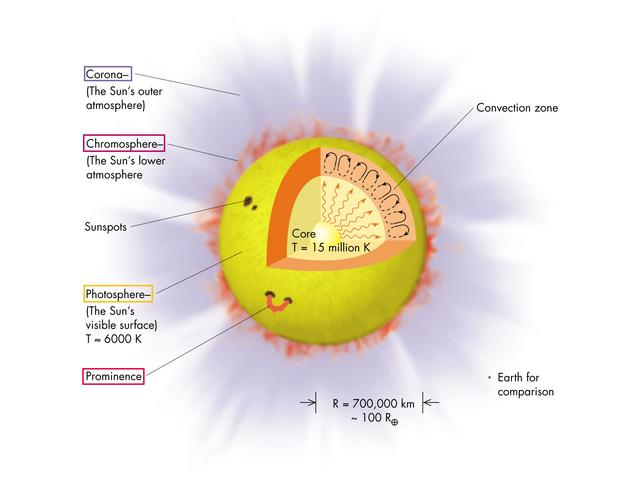
\includegraphics[trim = 0cm 0.5cm 0cm 0cm, width=1.0\textwidth]{images/solar_atmosphere}
\caption{The internal structure of the Sun, including the core, radiative zone, and convective zone.  Also shown is the structure of the its atmosphere, including the photosphere, chromosphere, and corona. The layers of the solar atmosphere are usually demarcated by temperature changes as height above the solar surface increases. The temperature ranges from $\sim$6000\,K in the photosphere to above 1\,MK in the corona.}
\label{fig:solar_atmosphere} 
\end{center}
\end{figure}

% Yuhong Fan, Living Reviews. "Because of the rapid decrease of the various scale heights in the top layer of the solar convection zone which demands increasing numerical resolution, it is not yet feasible to perform 3D MHD simulations that extend from the bottom of the convection zone all the way to the photosphere."

Much of what we know about the depth, temperature, and density of the convection zones come from a fine-tuning of the standard solar model, such that the model reproduces observations from neutrino and helioseismology experiments. In fact helioseismology alone can indicate great detail of the internal structure of the Sun. This field makes use of the fact the Sun acts as a resonator for acoustic waves which manifest as detectable oscillations in the doppler shift of photospheric Fraunhofer lines. These acoustic waves are referred to as pressure or p-modes, and a variety of wavelengths exist. Wavelengths that are an integer multiple of of the solar cavity may exist as standing wave modes. Such wave modes have a period of approximately 5 minutes \citep{turk2011}. 

\begin{figure}[!t]
\begin{center}
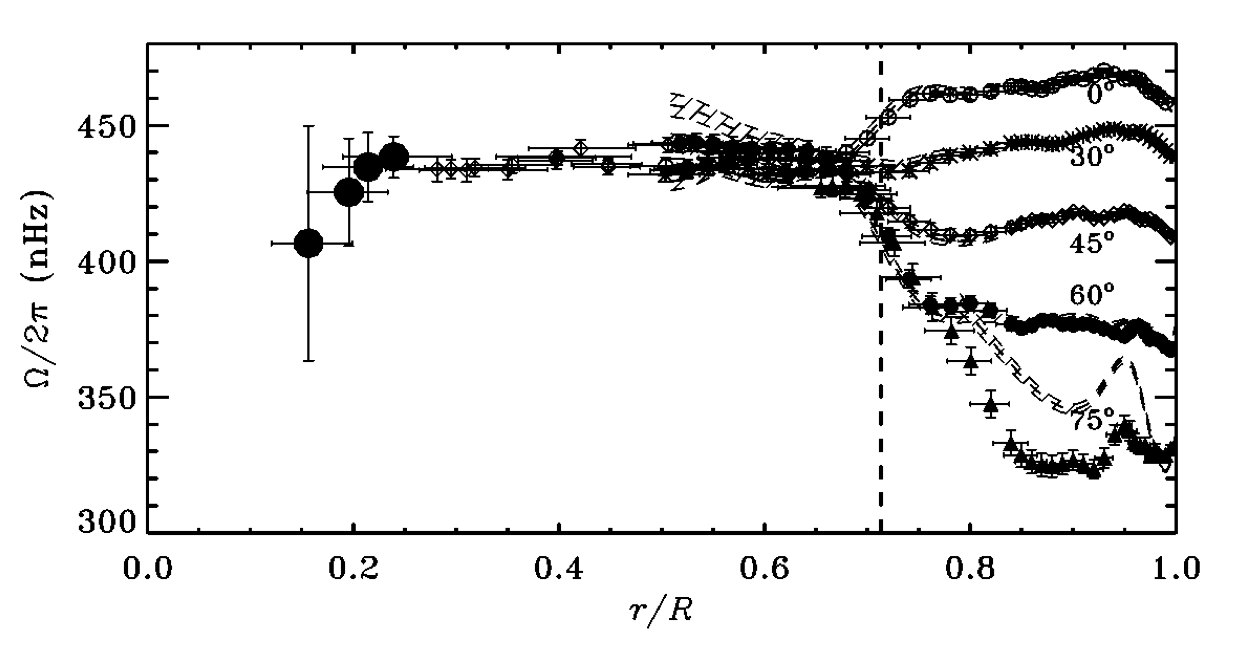
\includegraphics[trim = 0cm 0.5cm 0cm 0cm, width=1.0\textwidth]{images/differential_rot.png}
\caption{Helioseismological determination of interior rotation rate in nanoHertz (nHz) as a function solar radius, starting from solar centre ($r=0.0$) to surface ($r=1.0$). The separate symbols show different latitudes, from $0^{\circ}$ to $75^{\circ}$. The data show that the interior rotates differentially down to $\sim$$0.7\,R_{\odot}$. The dashed line demarcates the boundary between solid body rotation and differential rotation \citep{thompson2003}.}
\label{fig:diff_rot} 
\end{center}
\end{figure}


The shorter wavelengths in the mode propagate into the solar convection zone and experience a total internal reflection at a shallow depth, while longer wavelengths can penetrate into much deeper layers. Hence depending on the period observed, the oscillations provide a probe of the internal thermodynamic properties at a particular level. Once such property closely monitored is the sound speed, which is seen to match the predicted sound speed based on the standard model. However, the observation and prediction show the biggest deviation at a depth of $0.3\,R_{\odot}$, which is the region where the radiative zone transitions to the convective zone. This obviously implies that SSM is lacking in its description of how the solar interior is stratified at this depth. This partly due to the fact the SSM does not take into account differential rotation. The solar surface rotates faster at the equator than it does at the poles i.e., angular velocity is stratified with latitude. Helioseismology has revealed that such differential rotational continues to the bottom of the convection zone. In the deeper radiative zone and core the Sun rotates as a solid body see Figure~\ref{fig:diff_rot}. There is a dramatic change in the internal dynamics when transitioning from convective to radiative zones. 

As predicted by sound speed measurements and differential rotation, the region sandwiched in between radiative and convective zones is and extremely important boundary. It is known as the tachocline, and the dynamics of this thin layer is believed to play and extremely important role in the generation and evolution of the solar magnetic field \citep{thompson2003}.




\subsection{Solar Magnetic Field and Dynamo}\label{sec:11}

The solar magnetic field is the ultimately source of all energetic activity in the its atmosphere. At solar activity minimum the solar magnetic field has a poloidal dipolar structure, with the polar axes generally being coincident with the rotational axes. However as the the activity cycle progresses towards a maximum, the field gains a strong toroidal component, making it far more dynamic and complex. This complex toroidal component manifests at the surface as sunspots, hence the number of sunspots on disk has been used as a proxy for the activity cycle for over 100 years, often showing an approximate 11 year periodicity (Figure~\ref{fig:butterfly}, bottom panel). At the beginning of the cycle sunspots tend to appear on disk with a latitudinal distribution of $\pm30^{\circ}$ of the equator. As the cycle progresses, sunspots appear at lower and lower latitude (known as Sp\"{o}rer's law), until they eventually disappear at the end of a cycle. Sunspot latitude with respect to time is shown in Figure~\ref{fig:butterfly}, top panel, and is known as the butterfly diagram.

Sunspots in there simplest case emerge as a dipole structure, with the leading spot being closer to the equator, such that the dipole is titled relative to the solar equator (Joy's law). In a given hemisphere, the leading sunspot and trailing spot have opposite polarities, with the polarities reversed in the other hemisphere  (Hayle's law). The trailing polarity can often be more fragmented and dispersed that the leading polarity. Despite sunspots generally having a dipolar structure, spot groups can be far more complex, having a multipolar structure (this will be described more later).

Over the course of a solar cycle, the sun changes polarity (at the time of sunspot maximum). For example, an overall dipolar configuration of North-South will become South-North, another cycle will bring it back to N-S once more. While the activity cycle usually last 11 years, one full magnetic cycle has a period of 22 years.


\begin{figure}[!t]
\begin{center}
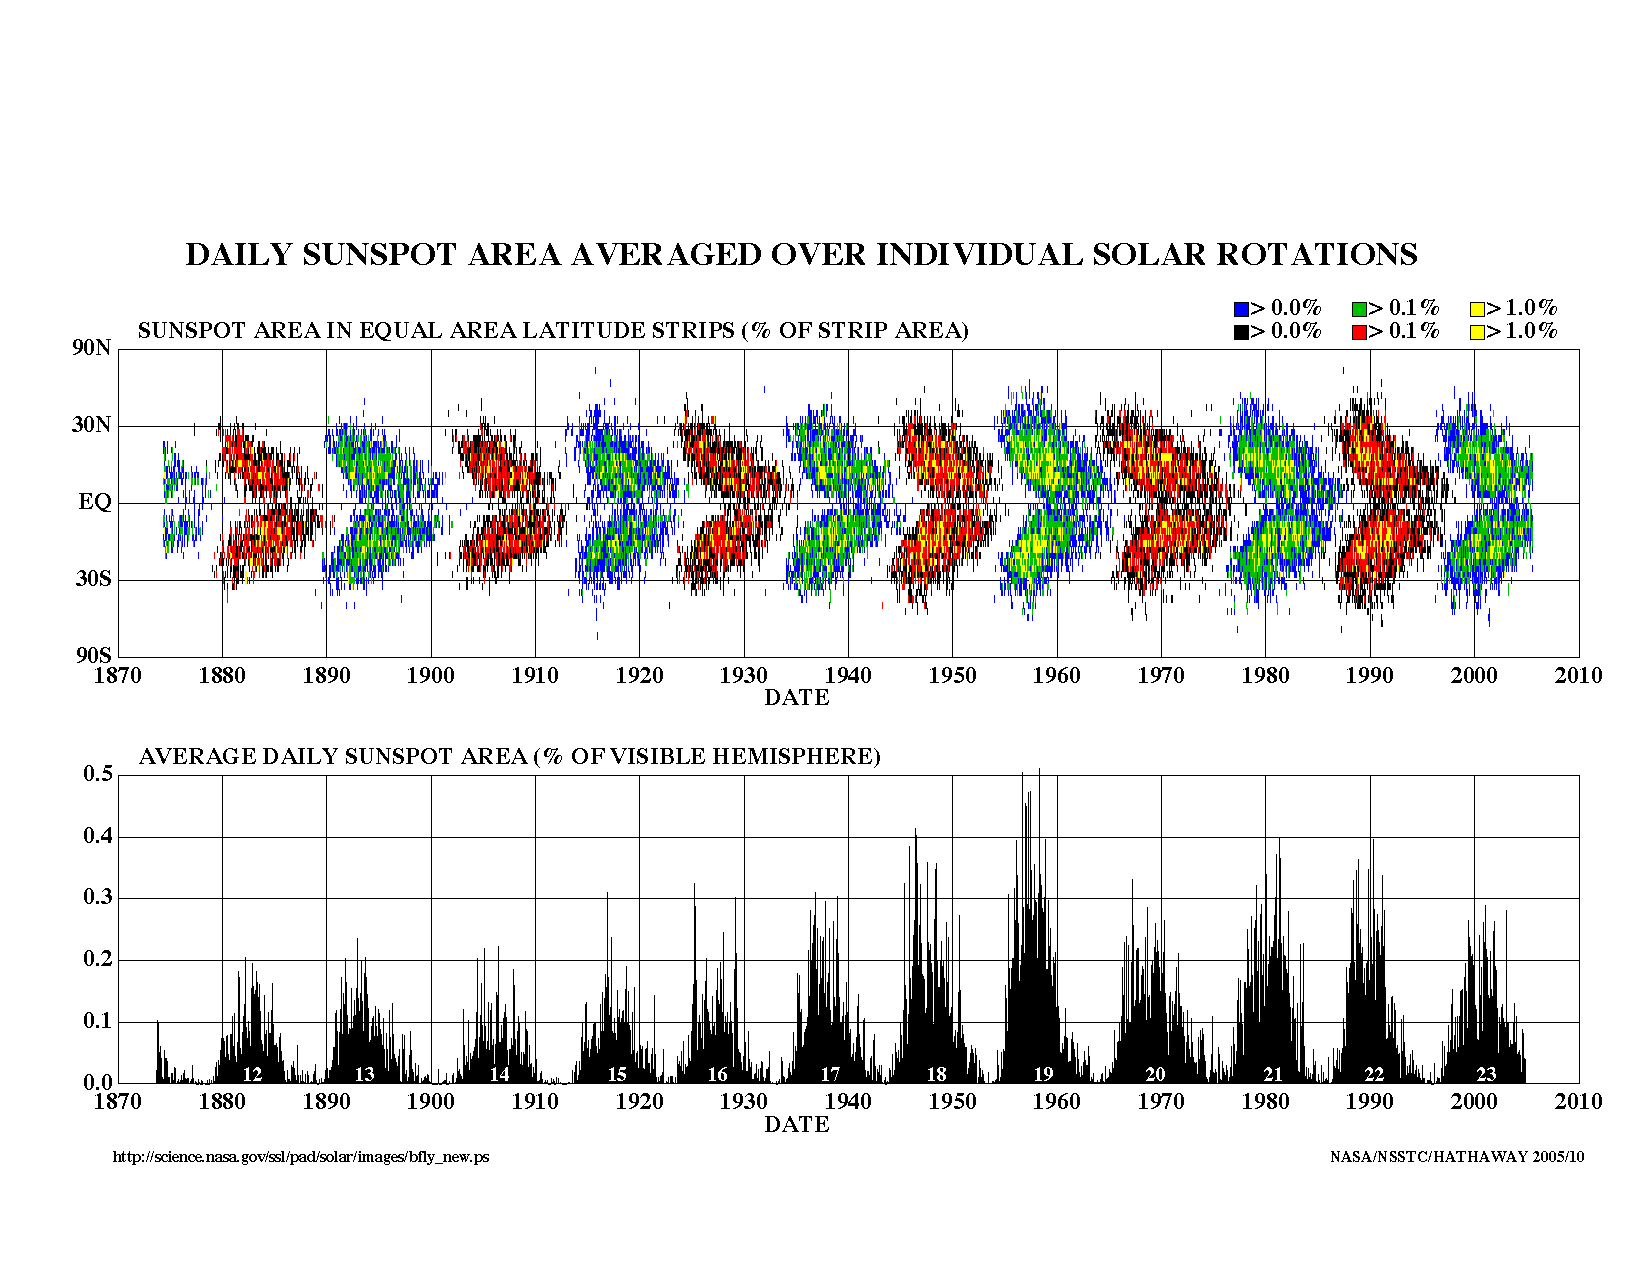
\includegraphics[scale=0.55, trim =1cm 1cm 0cm 3cm]{images/bfly_new.pdf}
\caption{Top: The latitude of sunspots as a function of time. During the rise phase of each cycle the sunspots have a latitudinal distribution of $\pm30^{\circ}$ from the equator.  As the solar cycle progresses, sunspots emergence takes place at an increasingly lower latitude. Bottom: Sunspot area as a function of time. The approximate 11 year periodicity is clearly shown.}
\label{fig:butterfly} 
\end{center}
\end{figure}


\begin{figure}[!h]
\begin{center}
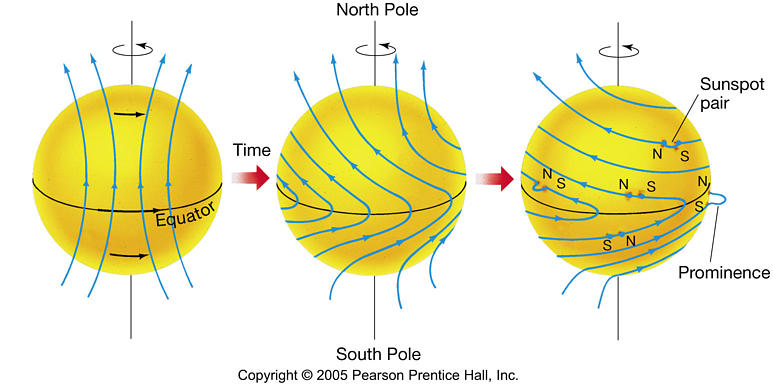
\includegraphics[]{images/Babcock}
\caption{Differential rotation and flux freezing result in the poloidal dipolar magnetic field, generated by dynamo action, to be dragged around in a toroidal direction, an action known as the omega effect. Buoyancy of the field lines results in them rising and twisting, known as the alpha effect, eventually surfacing to become bipolar fields that extend far into the corona.}
\label{fig:Babcock} 
\end{center}
\end{figure}

The complex behavior of the solar magnetic field over an 11 year activity cycle, during which the dipole flips, is generally explained by solar dynamo theory. This involves large-scale flow patterns of the solar interior that act to both induct and diffuse the magnetic field such that it produces the familiar 11 year magnetic activity cycle. Magnetohydrodynamics (MHD) is employed such that the magnetic induction equation and velocity field equation (equation of motion) are solved in numerical models to produce a toroidal field from a poloidal one, a process known as the $\Omega$-effect. The theories must adhere to the constraints provided by observations of the sunspot cycle (Sp\"{o}rer's, Joy's, and Hale's laws), and also helioseismology observations of how the interior is structured.


\citet{babcock1961} first proposed a mechanism whereby the differential rotation of the solar convection zone tends to drag the field from a poloidal position into a toroidal one, eventually winding the field into a a stressed state, see Figure~\ref{fig:Babcock}. The main storage of this wound field is in the region below the convection zone known as the tachocline. This region is known as an 'overshoot' layer, in which descending convective flows are a trapped due the subadiabicity of the region (convectively stable). This stability allows field to be built up and stored into complex magnetic structures. Parts of this structure may form a twisted magnetic 'flux-rope', and due to it's excess magnetic pressure, it becomes convectively unstable and begins to rise. During this rise a Coriolis force has a tendency to tilt into a north-south orientation and eventually penetrate through the solar surface and into the atmosphere, known as the $\alpha$-effect (the tilt from Coriolis effects explains Joy's law). Dynamo theory attempts to explain the $\Omega$-effect wrapping and build up of toroidal flux in the solar interior via inductive plasma flows \citep{charbon2010}, particularly using the observed flow structure from helioseismology. Further MHD of convective instabilities is employed to describe the $\alpha$-effect rise of flux systems into the solar atmosphere from the stably convective tachcoline/overshoot layer. This is very much a study in itself, and describes the eventual formation coronal active regions from sub-photospheric flux-systems \citep{fan2009}. 


\subsection{Solar Atmosphere}\label{sec:12}

The solar atmosphere begins above the visible surface of the sun, known as the photosphere. At this point, the Sun become optically thin to visible radiation and light escapes from this surface. Beyond this visible surface is the solar chromosphere, the corona, which eventually becomes the solar wind. Each of these layers is home to a complex array of phenomena, and each layer with it's accompanying attributes is described here.


\subsubsection{Photosphere}\label{sec:121}

As mentioned the photosphere begins where the atmosphere become optically thin. \textquoteleft Visible light' in this instance is usually taken to mean light with a wavelength of 5000\,\AA, hence the emergent light from the photosphere is taken to come from the surface at which $\tau_{5000}=2/3$. This is a consequence of the Eddington-Barbier approximation, and says that emergent flux $F_{\nu}$ from the photosphere is given by

\begin{equation}
F_\nu = \pi B_\nu(\tau=2/3)
\end{equation}
e.g., the emergent flux is given by $\pi$ times blackbody intensity at an optical depth of 2/3, where blackbody intensity $B_\nu$ is given by Planck's law 
\begin{equation}
B_\nu = \frac{2h\pi\nu^3}{c^2}\frac{1}{\mathrm{exp}(h\nu/k_BT)-1}
\end{equation}
where $h$ is Planck's constant, $\nu$ is frequency, $c$ is the speed of light, $k_B$ is Boltzmann's constant, and $T$ is temperature. Integrated over frequency this results in $F = \sigma T^4(\tau=2/3)$, where the frequency integrated flux is proportional to the temperature at $\tau=2/3$, hence the effective temperature of solar blackbody radiation is $T_{eff}=T(\tau=2/3)=5800$\,K. Solar radiation at visible wavelengths is most closely characterised by a blackbody of temperature 5800 K, although the brightness temperature $T_B$ the solar photosphere can deviate from this value, since not all frequencies emerge from the same optical depth.

The visible appearance of the photosphere reveals a small scale granular structure, with granules of typical size scale of 1000\,km with a lifetime of 5-10 minutes. The granules typically show bright centers surrounded by darker intergranular lanes. Doppler measurements reveal that granule centres have a positive (upward) velocity of up to $\sim1$\,km\,s$^{-1}$, with intergranular lanes having a negative (downward) velocity. Such upward and downward flow reveals that granulation at the photosphere are the surface manifestation of convective activity in the deeper layers of the sun, although the size scales of granules are much smaller than the convective plumes believed to permeate the convection zone. As well as the conspicuous granulation at the photospheric surface there is also a much larger scale \textquoteleft super-granulation' which has much the same mechanism as the granules e.g, upflows at granule centre and downflows at the edges in the granular network. The flow speeds are much slower with typical speeds of $0.1$\,km\,s$^{-1}$. The have a much larger size of $10,000-30,000$\,km and longer lifetimes of several days. They have an important role in the build up and concentration of magnetic flux in the intergranular lanes. Apart from, granules and supergranules, the most conspicuous features of the photosphere are sunspots. As discussed in the previous section, these are the surface manifestation of concentrated magnetic flux that has penetrated from the solar convective zone into the solar atmosphere. The spots have a temperature of $\sim4000$\,K, which is cooler than the typical solar blackbody temperature of $5800$\,K. The spots have typical magnetic field strengths of on the order of kilo-Gauss, and have an important role to play in solar activity.


Although the the intensity of the Sun in the visible may be approximated closely by a blackbody continuum, there are also the presence of dark absorption or Fraunhofer lines in the spectrum. The most notable of which are the H-alpha and Ca\Rmnum{2} H and K lines.  The presence of these lines reveals that cooler part of the photosphere must overly the hotter base at $\tau_{5000}=1$ \citep{phillips2008}. In fact, the variety of lines that are produced in the solar atmosphere (both emission and absorption) are used to determine the temperature and density stratification of the solar atmosphere.  That has most notably been done in the models of \citep{vernazza1981, fontenla1988, gabriel1976}, whereby a temperature and density profile of the solar atmosphere is used to calculate the emergent intensity, using radiative transfer theory. This temperature and density profile is adjusted until the the modeled emergent intensities match the observed ones. The results of this these models is shown in Figure~\ref{fig:val}. From this Figure we see that there is a temperature minimum at $\sim$500\,km above the photosphere where the temperature drops to $\sim$4400\,K. Beyond this point the temperature begins to rise again, eventually showing a rapid increase at $\sim$2000\,km. The region between the temperature minimum up the height at which temperature begins to rise rapidly is known as the chromosphere\footnote{These boundaries can vary, depending on the phenomenon observed e.g., spicules are chromospheric phenomenon which can extend far beyond the upper boundary of $\sim$2000\,km}. 

%About 15% of photospheric opacity is attributed to absorption features. The rest is H- opacity

\begin{figure}[!t]
\begin{center}
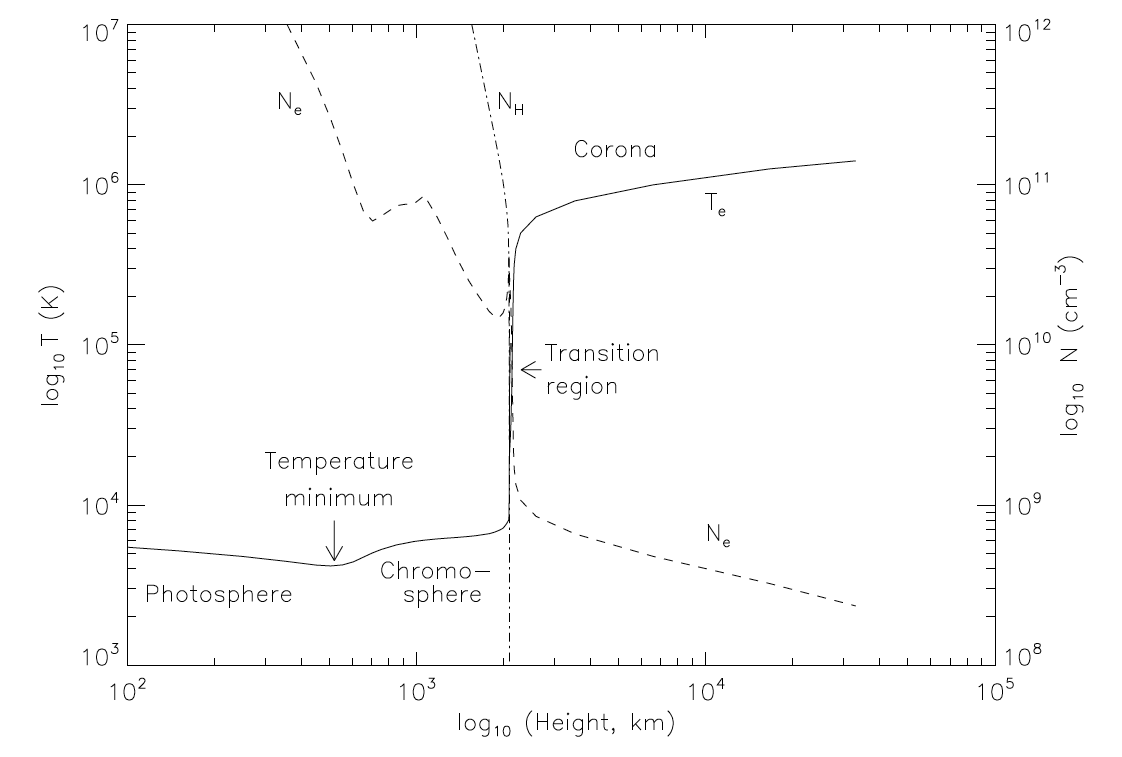
\includegraphics[scale=0.4]{images/VAL.png}
\caption{Temperature and density variation in the solar atmosphere constructed from the models of \citep{vernazza1981, fontenla1988, gabriel1976}, adopted from \citep{phillips2008}.}
\label{fig:val} 
\end{center}
\end{figure}


\subsubsection{Chromosphere}\label{sec:122}

\begin{itemize}
\item Appearance, Supergranular Network, Bright Points, Spicules, Filaments, Plage etc.
\item Emission lines, H-alpha, CaII H \& K. 
\item Temperature, Density, Opacity.
\item Magnetic field strength.
\end{itemize}

At $\sim$500\,km above the $\tau_{5000}=1$ surface the temperature drops to a minimum of $\sim$4400\,K. Beyond this minimum the temperature begins to rise again, demarcating the beginning of the chromosphere. This layer of the atmosphere is generally accepted to extend to a height at which temperatures reach 20,000\,K, however temperatures as high as $\sim1\times10^5$\,K are sometimes attributed to chromospheric heights, hence it is observable at ultraviolet (UV) wavelengths as well as visible. 

%Note: Fraunhofer lines such as Calcium H and K are not as simple as a case of a cloud of cooler gas absorbing lines from a hot radiations source. The Fraunhofer lines are a consequence of the Eddington-Barbier Approximation i.e., that the emergent intensity is equal to the source function at an optical depth of 2/3. So in the centre of the line the opacity goes up and optical depth 2/3 is higher in the atmosphere where the plasma is cooler. Hence, the line is darker at the centre (due to the smaller source function at the cooler temperature).

\subsubsection{Corona}\label{sec:123}

%Main characteristics of chromosphere are temperature increase with height, and constantly changing complex structure

%Details in the chromosphere are imaged using the lines of H-alpha and Ca II H and K. These Fraunhofer lines are formed over a large range in heights.

%The H-alpha line is photoelectrically controlled, so the decrease in line intensity is to do with the source function being lower because of a lack of photospheric photons at that height the line centre 'samples

%Ca II  H and K is collisionaly controlled so the decrease in line intensity is to do with the source function being lower because of the dropping temperature

%Different regions in the Ca II  H and K lines sample different heights in the photosphere/chromosphere. Tuning imagers to different parts of these lines allows imaging of chromosphere at different heights.

%Chromospheric lines not in the visible are the Mg h and k Fraunhofer lines, also collisionaly controlled. There is also the Ly-alpha emission line, formed at 20,000 K, which is optically thin. There is C IV, formed at 110,000 K, at this point we are starting to sample to transition region.


\begin{itemize}
\item Appearance UV: Active regions, Coronal Loops, Holes.
\item Emission lines, Mg, Ca, Fe, C, O etc.
\item Appearance White-Light: Streamers, K, F, E corona
\item Appearance Radio: thermal bremsstrahlung, free-free emissivity/opacity.
\item Temperature, Density, Opacity, 'coronal heating problem'.
\end{itemize}


At a height of approximately 2,000\,km the temperature begins to rise sharply while the number density of neutral hydrogen and electrons fall by several orders of magnitude. This rapid increase in temperature in such a short spatial extent ($<$100\,km) is known as the transition region. It has a temperature on the order of $10^5$\,K and separates the relatively low temperature chromosphere and the high temperatures of $>1$\,MK in the corona. The reason for this rapid increase in temperature is still a hotly debated subject and a coronal heating mechanism remains largely unknown, this is known as the  \textquoteleft coronal heating problem'.


Element abundances in the corona show there is a similar composition to the photospheric abundances, with He, C, N, and O having the same ratios relative to H in the corona as that in the photosphere. The only difference is an enhancement in the abundance of low First Ionization Potential ($<10$\,eV) elements in the corona relative to the photosphere. For example, elements such as Na, Mg, Al, Si, Ca, Ni, and Fe can be up to three times more abundant in the corona \citep{feldman2003}. The reason for the enhancement of low FIP elements in the corona is still unknown, however several models have suggested ion-neutral separation in the chromosphere by diffusion across magnetic fields, followed by transport of these ions into the corona may be viable mechanism \citep{geiss1985}. 


\subsection{Solar Wind}\label{sec:13}

\begin{itemize}
\item Parker's solution
\item Parker Spiral
\item Fast solar wind, Alfv\'{e}n wave driver
\item Mass loss rates (later compare CME mass loss)
\end{itemize}



\section{Coronal Mass Ejections and Coronal Shocks}\label{sec:2}

\subsection{CMEs}\label{sec:20}

\begin{itemize}
\item Appearance, white-light Illing, Hundhausen, Vourlidas
\item Kinematics, velocity, acceleration
\item Dynamics, masses, energies, forces
\item Observations at other wavelengths, EUV, radio, SXR.
\end{itemize}

\subsection{CMEs and Shocks}\label{sec:21}

\begin{itemize}
\item Radio bursts, Type II, Type III
\item Radio imaging of shocks
\item Relationship to EUV waves, Moreton waves
\end{itemize}

\subsection{Open Questions}\label{sec:22}






